\documentclass{lecturenotes-sta}
\begin{document}
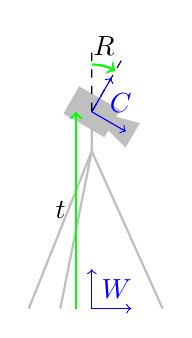
\begin{tikzpicture}

\draw[thick, lightgray]
    (0, 2.0) -- ( .9, 0)
    (0, 2.5) -- ( 0., 2) -- (-0.4, 0)
    (0, 2.0) -- (-.8, 0);

\begin{scope}[shift={(0,2.5)},rotate=-30]
\fill[lightgray]
    (-.3, .2 ) -- (.3, .2) -- (.3, .1) -- ( .6, .18) --
    ( .6,-.18) -- (.3,-.1) -- (.3,-.2) -- (-.3,-.2 ) -- cycle;
\end{scope}

\begin{scope}[shift={(0,2.5)},rotate=-30, shift={(0,0)}]
\coordinate (a) at (0,0);
\draw[dashed] (120:.75) -- ++ (-60:.75) ++ (0,.75) -- (0,0);
\draw[->,thick,green]
    (120:0.6) arc[radius=.6, start angle=120, end angle={90}]
    node[pos=0.5, above, black] {\(\matr{R}\)};

\draw[<->, blue]
    (0,.5) -- (0,0) -- + (.5,0)
    node[pos=0, right, shift={(3pt,3pt)}] {\(\symcal{C}\)};
\end{scope}

\draw[->,thick,green, xshift=-2mm]
    (0,0) -- ++ (0,2.5) node[pos=0.5, left, black] {\(\vect{t}\)};

\draw[<->, blue]
    (0, .5) -- (0,0) -- (.5, 0)
    node[pos=0, above right] {\(\symcal{W}\)};

\end{tikzpicture}
\end{document}
